%%%%%%%%%%%%%%%%%%%%%%%%%%%%%%%%%%%%%%%%%
% Beamer Presentation
% LaTeX Template
% Version 1.0 (10/11/12)
%
% This template has been downloaded from:
% http://www.LaTeXTemplates.com
%
% License:
% CC BY-NC-SA 3.0 (http://creativecommons.org/licenses/by-nc-sa/3.0/)
%
%%%%%%%%%%%%%%%%%%%%%%%%%%%%%%%%%%%%%%%%%

%----------------------------------------------------------------------------------------
%	PACKAGES AND THEMES
%----------------------------------------------------------------------------------------

\documentclass{beamer}

\mode<presentation> {
  \usetheme{Madrid}
}

\usepackage{graphicx}
\usepackage{booktabs}
\usepackage[utf8]{inputenc}

%------------------------------------------------------------------------------%
%                                  TITLE PAGE                                  %
%------------------------------------------------------------------------------%

\title[SWAP-IFC]{Secure Web Applications with Information Flow Control}

\author{Alexander Sjösten}
\institute[GU]
{
Master's Thesis in Computer Science \\
\medskip
Examiner: Andrei Sabelfeld 
}
\date{\today}

\begin{document}

\begin{frame}
\titlepage
\end{frame}

%------------------------------------------------------------------------------%
%                             PRESENTATION SLIDES                              %
%------------------------------------------------------------------------------%

\begin{frame}
  \frametitle{Security issues in web applications}
  \begin{itemize}
    \item Many ways an attacker can gain access to information. \pause
    \item Cross Site Scripting (XSS) attacks ranked nr. 3 on OWASP Top 10 list. \pause
    \item Usual culprits: non-escaped user input. \pause
    \item Harmless pranks (show alert box) to redirecting to fake website to steal valuable information.
  \end{itemize}
\end{frame}

%------------------------------------------------------------------------------%

\begin{frame}[fragile]
  \frametitle{JavaScript is bad!}
  Weak typing.
  \begin{block}{}
\begin{verbatim}
var age = prompt("What is your age?", "");
console.log(
    "You are now " + age + " years old. In 20 years you are " +
   (age + 20) + " years old!"
);
\end{verbatim}
  \end{block}
  What will the output be if 20 is the input??\pause \emph{"You are now 20 years old. In 20 years you are 2020 years old!"}
  \pause
  \newline
  Access to sensitive information (cookies, session tokens) in the browser. \pause
  Crucial to ensure information can not be leaked.
\end{frame}

%------------------------------------------------------------------------------%

\begin{frame}
  \frametitle{Tools used}
  JSFlow, a dynamic system for ensuring information flow control. \pause
  \newline
  JSFlow supports ECMA-262 v5, except for JSON and strict mode. \pause
  \newline
  \newline
  Haste, a compiler from Haskell to JavaScript. \pause
  \newline
  Ensures type safe JavaScript code. \pause
  \newline
  \newline
  Goal of the project is to extend Haste to produce JavaScript code targeting JSFlow.
\end{frame}

%------------------------------------------------------------------------------%


\begin{frame}
  \frametitle{Information flow control}
  Normally, applications in e.g. JavaScript has one input channel and one output channel.
  \begin{figure}[h]
    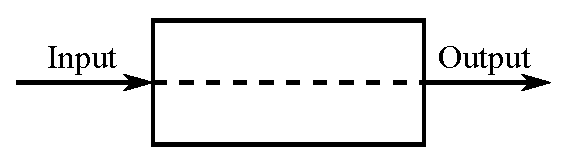
\includegraphics[scale=0.65]{images/flow_normal.eps}
  \end{figure}
  \pause
  Information flow control defines which flows are valid.
  \begin{figure}[h]
    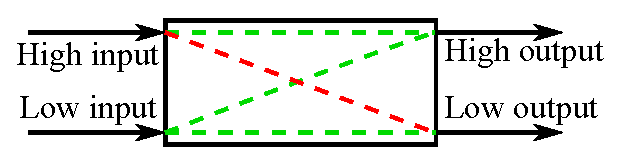
\includegraphics[scale=0.65]{images/flow_controlled.eps}
  \end{figure}
\end{frame}

%------------------------------------------------------------------------------%

\begin{frame}[fragile]
  \frametitle{Different flows}
  Two types of flows, \textbf{explicit} and \textbf{implicit} flows \pause
  \newline
  \begin{block}{Explicit flow}
\begin{verbatim}
  l := h;
\end{verbatim}
  \end{block}
  Private value is assigned \emph{directly} to a public variable.
  \pause
  \begin{block}{Implicit flow}
\begin{verbatim}
  h := h `mod` 2
  l := 0;
  if h == 1 then
      l := 1;
    else
      skip;
\end{verbatim}
  \end{block}
  Information of private values are leaked through \emph{indirectly} through e.g. control structures.
\end{frame}

%------------------------------------------------------------------------------%

\begin{frame}[fragile]
  \frametitle{Non-interference}
  Public output does not depend on private input. \pause

  \begin{block}{Function fullfilling non-interference}
\begin{verbatim}
f :: (Char, Int) -> (Char, Int)
f (c, i) = (chr (ord c + i), i + 42)
\end{verbatim}
  \end{block}
  \pause
  \begin{block}{Function not fullfilling non-interference}
\begin{verbatim}
f' :: (Char, Int) -> (Char, Int)
f' (c, i) = (c, ord c)
\end{verbatim}
  \end{block}
  \pause
  Information about the secret character (its ASCII value) is being leaked.
  \pause
  \newline
  However, a system satisfying non-interference is very strict...
\end{frame}

%------------------------------------------------------------------------------%

\begin{frame}
  \frametitle{Declassification}
  Sometimes it is necessary to release some private information.\pause
  \newline
  Imagine a login system. \pause
  \begin{itemize}
    \item User inserts username and password.
    \item Username is public data (i.e. low) and passwords are private data (i.e. high).
    \item If the username and password matches, the user is redirected.
    \item If the username and password does not match, message is shown to the user.
  \end{itemize}
  \pause
  If the system was non-interfered, no information would be given to the user.\pause
  \newline
  Declassification is used to "downgrade" a value from a secure context to a less secure context. \pause
  \newline
  Can be classified as four dimensions: \textbf{who}, \textbf{what}, \textbf{when}, \textbf{where}.
\end{frame}

%------------------------------------------------------------------------------%

\begin{frame}[fragile]
  \frametitle{Examples of coding for JSFlow}
  Two important functions, \textbf{upg} and \textbf{declassify}.
  \pause
  \begin{block}{Upgrading a value}
\begin{verbatim}
var l = 10;
var h = upg(42);
\end{verbatim}
  \end{block}
  \textbf{l} will be a \emph{low} value, \textbf{h} will be a \emph{high} value.
  \pause
  \begin{block}{Downgrading a value}
\begin{verbatim}
var h = upg(42);
var l = declassify(h);
\end{verbatim}
  \end{block}
  \textbf{l} will be a \emph{low} value, containing the same value as \textbf{h}.
\end{frame}

%------------------------------------------------------------------------------%

\begin{frame}[fragile]
  \frametitle{SwapIFC - The library}
  \begin{itemize}
    \item Two different Monad, Applicative and Functor instances. In particular, \textbf{return} differs. \pause
    \item Implementation of primitives for \textbf{Bool}, \textbf{Num}, \textbf{Frac}, \textbf{Ord} and \textbf{Eq} classes. \pause
\begin{verbatim}
Flow Low 10 .+. Flow Low 20 ==> Flow Low 30
\end{verbatim}
\pause
    \item Unsafe functions for \textbf{declassify} and \textbf{unwrap} a value. \pause
    \item Supports side effects.
  \end{itemize}
\end{frame}

%------------------------------------------------------------------------------%

\begin{frame}[fragile]
  \frametitle{SwapIFC - The library}
  \begin{block}{Flow type}
\begin{verbatim}
newtype Flow tag a = Flow (IO a)
\end{verbatim}
  \end{block}
  {\tt tag} is a phantom type, i.e. lives only in the type system. \pause
  \begin{block}{Class implementations}
\begin{verbatim}
class FlowBool t1 t2 t3 | t1, t2 -> t3 where
-- function implementations for boolean operators

instance FlowBool High High High
instance FlowBool High Low High
instance FlowBool Low High High
instance FlowBool Low Low Low
\end{verbatim}
  \end{block}
  Uses functional dependencies to define how {\tt t1} and {\tt t2} relates to {\tt t3}.
\end{frame}

%------------------------------------------------------------------------------%

\begin{frame}
  \frametitle{Side effects}
  JSFlow keeps track of \emph{program counter label} ({\tt pc}) which reflects security level. \pause
  \newline
  Within every guarded expression, it must hold that:\[ \forall ge \in GuardedExpressions: ge_c \geq pc \] \pause
  If \emph{pc} is high, all modified \emph{ge} must be high. If \emph{pc} is low, \emph{ge} can be either high or low.
\end{frame}

%------------------------------------------------------------------------------%

\begin{frame}[fragile]
  \frametitle{Side effects}
  SwapIFC implements side effects with IORefs:
  \begin{block}{SwapIFC side effects}
\begin{verbatim}
newtype FlowRef tag a = FlowRef (IORef a)

newFlowRef :: a -> Flow t (FlowRef t a)
readFlowRef :: FlowRef t a -> Flow t a
writeFlowRef :: FlowRef t a -> a -> Flow t ()
modifyFlowRef :: FlowRef t a -> (a -> a) -> Flow t ()
\end{verbatim}
  \end{block}
  \pause
  Handling side effects in SwapIFC stricter compared to JSFlow, tag of {\tt FlowRef} must be the same as the {\tt Flow}.
\end{frame}

%------------------------------------------------------------------------------%

\begin{frame}[fragile]
  \frametitle{Integrating SwapIFC with Haste}
  Use preprocessor directives to know if Haste is the compiler:
  \begin{block}{}
\begin{verbatim}
-- High Monad instance
#ifdef __HASTE__
  return = Flow . upg
#else
  return = Flow . return
#endif
\end{verbatim}
  \end{block}
  \pause
  Call special utility functions if Haste is the compiler.
\end{frame}

%------------------------------------------------------------------------------%

\begin{frame}[fragile]
  \frametitle{Communicating with JSFlow}
  Use Foreign Function Interface (FFI)
  \begin{block}{}
\begin{verbatim}
-- Have JavaScript code call upg in JSFlow
upg :: a -> IO a
upg = fmap fromOpaque . ffi "upg" . toOpaque

-- Have JavaScript code call lprint in JSFlow
lprintHaste :: Show a => a -> IO ()
lprintHaste = ffi "(function(x) { lprint(x); })" . show
\end{verbatim}
  \end{block}
  \pause
  Uses anonymous function for {\tt lprintHaste}. Otherwise, edge case in the static runtime code from Haste is triggered.
\end{frame}

%------------------------------------------------------------------------------%

\begin{frame}
  \frametitle{Demo!}
  \centering
  \Huge \textbf{DEMO!}
\end{frame}

%------------------------------------------------------------------------------%

\begin{frame}[fragile]
  \frametitle{Testing}
  \begin{itemize}
    \item Write the erroneous type signatures for each primitve. Compile error. \pause
\begin{verbatim}
  badFlow1 :: Num a
           => Flow High a
           -> Flow Low a
           -> Flow Low a
  badFlow1 = (.+.)
\end{verbatim}
\pause
    \item Unit testing. \pause
    \item Randomized testing with QuickCheck. \pause
      \begin{itemize}
        \item For every class (e.g. FlowNum), generate primitive and values. \pause
        \item Create flows using values. \pause
        \item Perform operation with values, check if correct. \pause
        \item Tag is only in type system. \pause Unsafe operations to the rescue! \pause
        \item Repeat 100000 times for every combination. \pause Result: No errors!
      \end{itemize}
  \end{itemize}
\end{frame}

%------------------------------------------------------------------------------%

\begin{frame}
  \frametitle{Conclusion}
  \begin{itemize}
    \item Library for static information flow control. \pause
    \item Non-interference is guaranteed if no unsafe operations are used. \pause
    \item Generates valid code for JSFlow w.r.t. low flows. \pause
    \item Can handle side effects.
  \end{itemize}
\end{frame}

%------------------------------------------------------------------------------%

\begin{frame}
  \frametitle{Future work}
  As with everything, nothing is perfect. \pause
  \begin{itemize}
    \item Implement full support for JSFlow (i.e. support High flows) and test the code generation. \pause
    \item End-to-end communication, including Haste.App and databases etc. \pause
    \item More features for JSFlow, including JSON and browser support. \pause
    \item More primitives for SwapIFC.
  \end{itemize}
\end{frame}

%------------------------------------------------------------------------------%

\begin{frame}
  \frametitle{The end!}
  \Huge
  \begin{center}
    Thank you!
  \end{center}
  \begin{center}
    Questions?
  \end{center}
\end{frame}

%------------------------------------------------------------------------------%

\end{document}
